\documentclass[12pt,a4paper]{report}
\usepackage[utf8]{inputenc}
\usepackage[spanish]{babel}
\usepackage{geometry}
\geometry{a4paper, margin=2.54cm}
\usepackage{hyperref}
\usepackage{longtable}
\usepackage{booktabs}
\usepackage{graphicx}
\usepackage{float}

\title{Análisis Reto: GIRO \\ Sistema de Gestión de Inventario y Pedidos}
\author{Hansell Steven Benavides Jumbo - Sergi Montaño Galarza}
\date{\today}

\begin{document}
	
	\maketitle
	\tableofcontents
	\newpage
	
	\chapter{Capítulo 1: Introducción y Problemática}
	
	\section{Introducción}
	El presente documento tiene como propósito definir la visión general del Sistema de Gestión de Inventario y Pedidos B2B, denominado GIRO. Este sistema se establece en el contexto de la distribución mayorista, abarcando la atención de micromercados (tiendas pequeñas) en zonas tanto rurales como urbanas del Ecuador. Su objetivo principal es optimizar la vinculación comercial entre proveedores mayoristas y vendedores en ruta, reducir la pérdida de ventas mediante control de inventario en tiempo real y automatizar la toma de pedidos.
	
	\section{Problemática}
	La problemática central radica en la desconexión operativa entre el inventario real disponible de los proveedores mayoristas y la gestión de campo realizada por los vendedores en ruta al visitar micromercados. Los vendedores a menudo operan con información desactualizada, lo que genera pedidos sobre productos agotados, compromisos de entrega incumplidos y pérdidas financieras. Adicionalmente, la falta de un canal digital estructurado dificulta la gestión de solicitudes de vinculación comercial y el seguimiento del estado de los pedidos por parte de las tiendas pequeñas.
	
	\section{Metodología o estrategia de desarrollo}
	La estrategia de desarrollo se apoya en iteraciones ágiles, validación continua con stakeholders y la ejecución de \textit{sprints} de refinamiento junto al equipo de desarrollo. Se incorporan también prácticas de análisis de negocio basadas en estándares del BABOK.
	
	A nivel de arquitectura técnica, el proyecto utilizará \textbf{sqlite} como motor de base de datos relacional. Se seleccionó sqlite por su alta escalabilidad y la facilidad de implementación con el equipo actual. Para el desarrollo del backend, se empleará el framework \textbf{Django} (Python), el cual permite desarrollar de forma rápida, estructurada y segura la API REST que sirve de soporte tanto a la aplicación web (PWA) de los vendedores como a los paneles de gestión de los proveedores.
	
	\chapter{Capítulo 2: Planificación y análisis}
	
	\section{Análisis de Actores y Modelo de Negocio}
	El análisis del sistema actual redefine el flujo operativo en torno a tres roles principales definidos en la arquitectura de datos:
	\begin{itemize}
		\item \textbf{Proveedor (Mayorista):} Dueño de los productos e inventario. Administra su catálogo, aprueba solicitudes de incorporación de vendedores y gestiona el ciclo de vida de los pedidos.
		\item \textbf{Vendedor:} Actor en ruta que explora proveedores verificados, envía solicitudes de asociación y registra pedidos en representación de las tiendas pequeñas, calculando sus comisiones.
		\item \textbf{Tienda Pequeña (Micromercado):} Negocio local que interactúa mediante solicitudes de visita o recepción de pedidos gestionados por su vendedor asignado.
	\end{itemize}
	
	\section{Requisitos funcionales}
	A continuación, se listan los requisitos funcionales principales extraídos del análisis y adaptados a la arquitectura de la base de datos:
	\begin{itemize}
		\item \textbf{RF-01 (Gestión de Catálogo):} El sistema debe permitir al \textit{Proveedor} registrar, actualizar y eliminar productos con control automático de SKU, stock disponible y precios.
		\item \textbf{RF-02 (Asociación de Vendedores):} El \textit{Vendedor} debe poder explorar proveedores verificados, enviar una solicitud de vinculación con una descripción de intenciones y esperar la aprobación y asignación de comisión por parte del mayorista.
		\item \textbf{RF-03 (Toma de Pedidos en Ruta):} El \textit{Vendedor} debe poder iniciar un pedido seleccionando una \textit{Tienda}, agregando productos del catálogo del proveedor asociado y registrando el método de pago (Efectivo o Transferencia).
		\item \textbf{RF-04 (Seguimiento y Ciclo del Pedido):} El \textit{Proveedor} debe poder avanzar el estado del pedido de forma secuencial (\textit{'En proceso' $\rightarrow$ 'Enviado' $\rightarrow$ 'En ruta' $\rightarrow$ 'Entregado'}).
		\item \textbf{RF-05 (Solicitud de Visitas):} Las \textit{Tiendas pequeñas} deben poder enviar solicitudes de visita a los vendedores de su sector para coordinar la reposición de inventario.
	\end{itemize}
	
	\section{Requisitos no funcionales}
	Los requisitos de calidad técnica y restricciones operativas incluyen:
	\begin{itemize}
		\item \textbf{RNF-01 (Seguridad y Control de Acceso - RBAC):} El acceso a los diferentes módulos debe restringirse estrictamente mediante autenticación de Django y validación de perfiles (\texttt{perfil\_proveedor}, \texttt{perfil\_vendedor}), aplicando el principio de mínimo privilegio.
		\item \textbf{RNF-02 (Rendimiento):} La búsqueda y filtrado de productos en el catálogo del proveedor mediante consultas optimizadas (\textit{icontains}) debe resolverse en el servidor en menos de 1.5 segundos.
		\item \textbf{RNF-03 (Seguridad en Tránsito):} Toda comunicación debe realizarse mediante HTTPS con TLS 1.3.
		\item \textbf{RNF-04 (Integridad de Datos):} Las operaciones críticas de inventario, creación de pedidos y aprobación de solicitudes deben ejecutarse bajo transacciones atómicas del ORM de Django para evitar inconsistencias relacionales.
		\item \textbf{RNF-05 (Disponibilidad):} Garantizar un \textit{uptime} mínimo del 99.5\% mensual.
	\end{itemize}
	
	\section{Historias de Usuario / Casos de Uso}
	En esta sección se modela la interacción entre los actores del sistema GIRO y las funcionalidades principales mediante diagramas de casos de uso orientados a los tres roles reales de la plataforma.
	
	\begin{figure}[H]
		\centering
		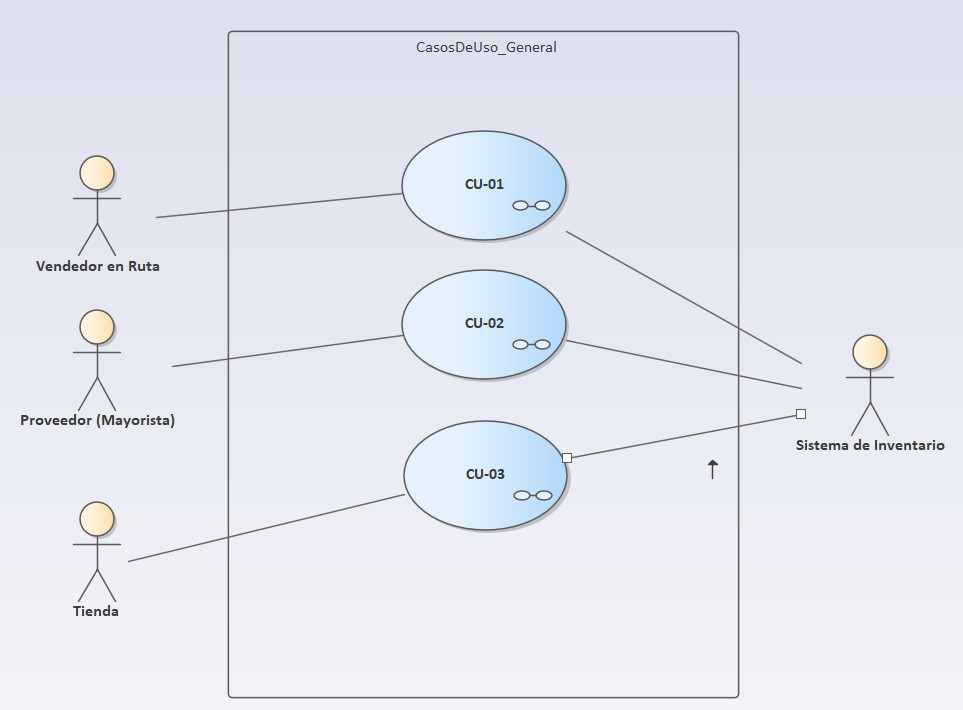
\includegraphics[width=0.8\textwidth]{cap_uno.jpg}
		\caption{Diagrama de Casos de Uso General}
		\label{fig:cu_general}
	\end{figure}
	En la Figura \ref{fig:cu_general} se ilustra la visión global del sistema. Se identifican los actores actualizados (Proveedor, Vendedor y Tienda Pequeña) interactuando con los módulos centrales de gestión y transaccionalidad.
	
	\begin{figure}[H]
		\centering
		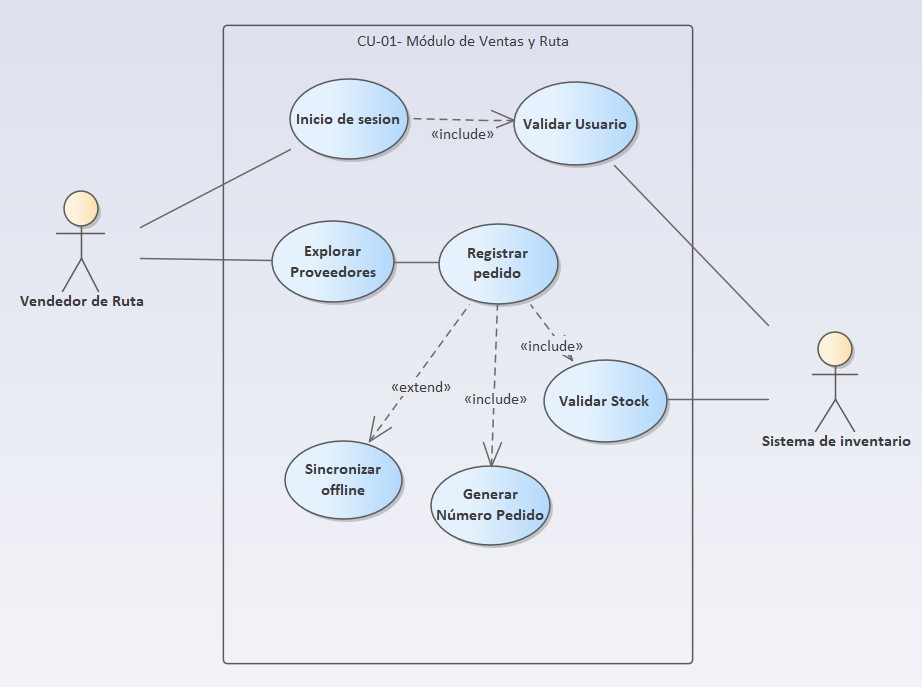
\includegraphics[width=0.8\textwidth]{cap_dos.jpg}
		\caption{Flujo Principal: Registro de pedido en campo}
		\label{fig:cu_01_a}
	\end{figure}
	La Figura \ref{fig:cu_01_a} detalla el Caso de Uso de toma de pedidos. Aquí se observa cómo el Vendedor inicia sesión con su perfil validado y procede a procesar el pedido vinculado a la tienda correspondiente.
	
	\begin{figure}[H]
		\centering
		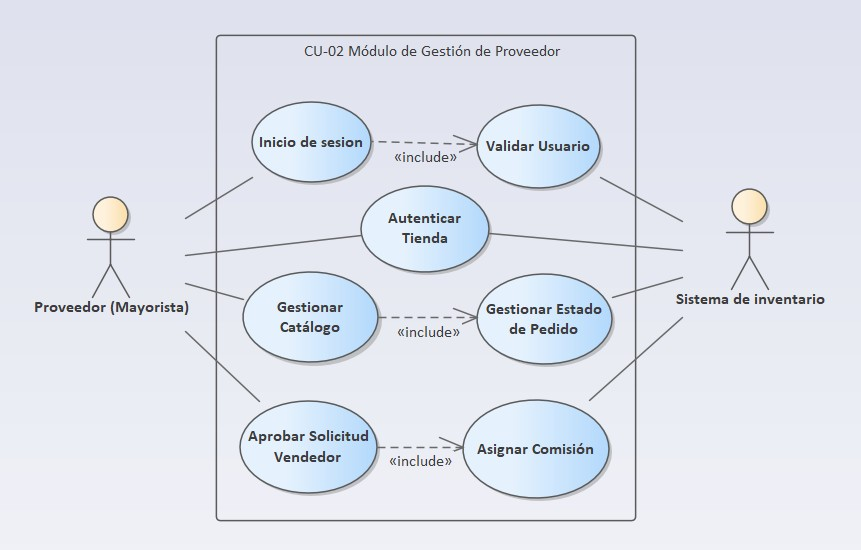
\includegraphics[width=0.8\textwidth]{cap_tres.jpg}
		\caption{Validaciones del Registro de Pedido}
		\label{fig:cu_01_b}
	\end{figure}
	Como se detalla en la Figura \ref{fig:cu_01_b}, el registro del pedido tiene dependencias estrictas (\textit{includes}): requiere validar el stock disponible en el catálogo del proveedor y verificar la existencia de una relación comercial activa.
	
	\begin{figure}[H]
		\centering
		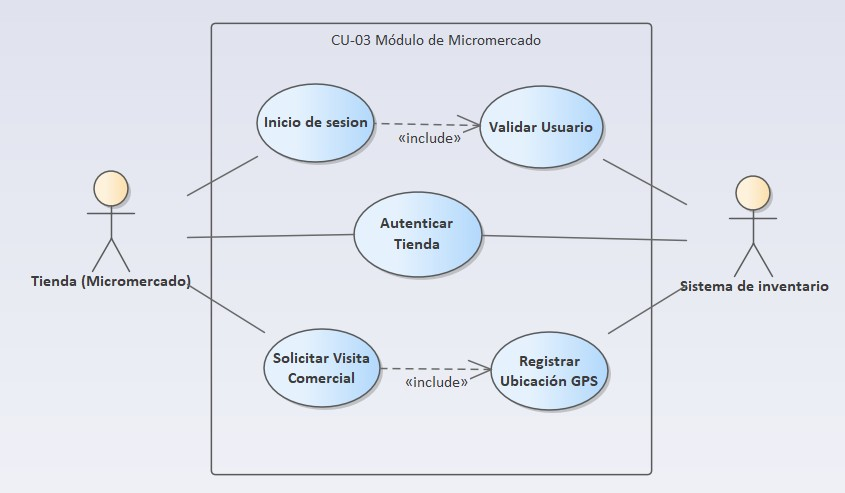
\includegraphics[width=0.8\textwidth]{cap_cuatro.jpg}
		\caption{Extensión Offline del Registro de Pedido}
		\label{fig:cu_01_c}
	\end{figure}
	Finalmente, la Figura \ref{fig:cu_01_c} resalta la funcionalidad \textit{extend} del sistema: en caso de que el vendedor se encuentre en una zona rural sin cobertura, el sistema extiende su comportamiento para habilitar el almacenamiento local cifrado, sincronizando posteriormente los datos al recuperar la señal.
	
	\section{Sprint}
	La estrategia de desarrollo se divide en iteraciones o \textit{Sprints} enfocados en entregar valor incremental alineado a los módulos críticos del sistema:
	\begin{itemize}
		\item \textbf{Sprint 1: Base, Autenticación y Catálogo.} Configuración de la base de datos MariaDB, despliegue del backend en Django, control de acceso basado en roles (RBAC) y la gestión de productos por parte del Proveedor.
		\item \textbf{Sprint 2: Módulo Web de Campo y Venta.} Desarrollo de la interfaz para vendedores, flujo de exploración de proveedores, envío de solicitudes de vinculación y el registro operativo de pedidos para las tiendas.
		\item \textbf{Sprint 3: Supervisión, Estados y Logística.} Implementación de la gestión de estados de pedidos por parte del mayorista (\textit{En proceso, Enviado, En ruta, Entregado}) y el submódulo de solicitudes de visita.
	\end{itemize}
	
	\section{Diagramas: Clases y BD (diseño lógico)}
	A continuación, se presenta el diseño estructural del sistema, alineado de forma estricta con la implementación real del código backend (\texttt{models.py}).
	
	\begin{figure}[H]
		\centering
		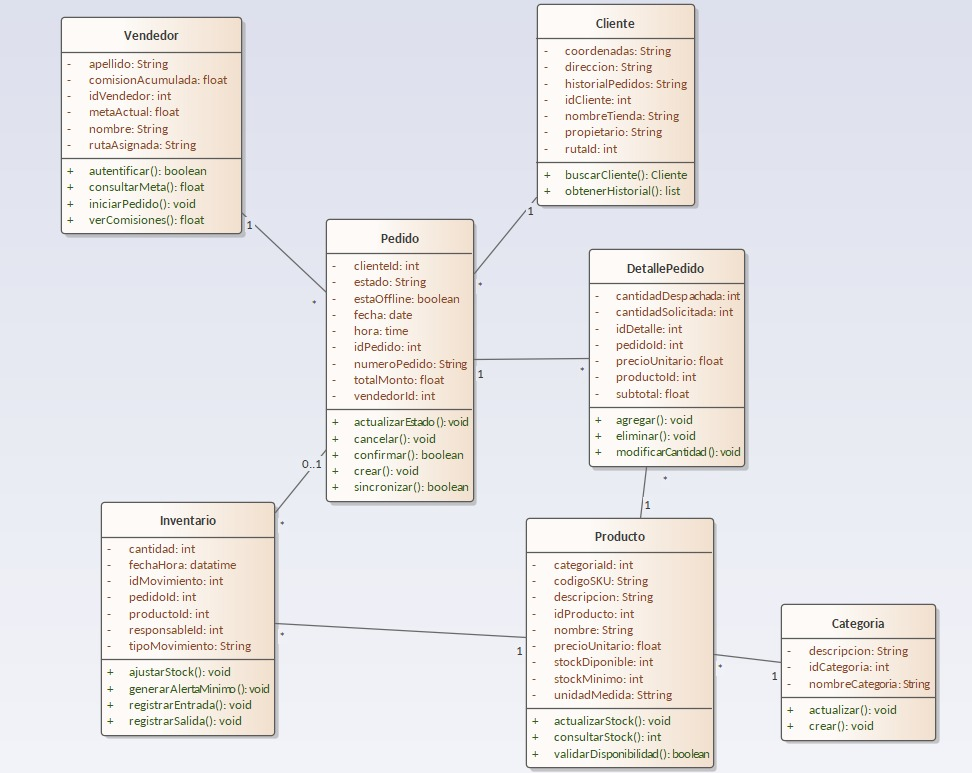
\includegraphics[width=0.9\textwidth]{Diagrama_Clases.jpg}
		\caption{Diagrama de Clases (Lógica de Negocio)}
		\label{fig:diagrama_clases}
	\end{figure}
	La Figura \ref{fig:diagrama_clases} muestra el diagrama de clases de UML actualizado. Este modelo define las entidades principales del dominio: \texttt{User}, \texttt{Proveedor}, \texttt{Vendedor}, \texttt{Tienda}, \texttt{SolicitudVendedor}, \texttt{Producto}, \texttt{Categoria}, \texttt{Pedido}, \texttt{DetallePedido} y \texttt{SolicitudVisita}, detallando sus atributos y métodos de operación conforme al ORM.
	
	\begin{figure}[H]
		\centering
		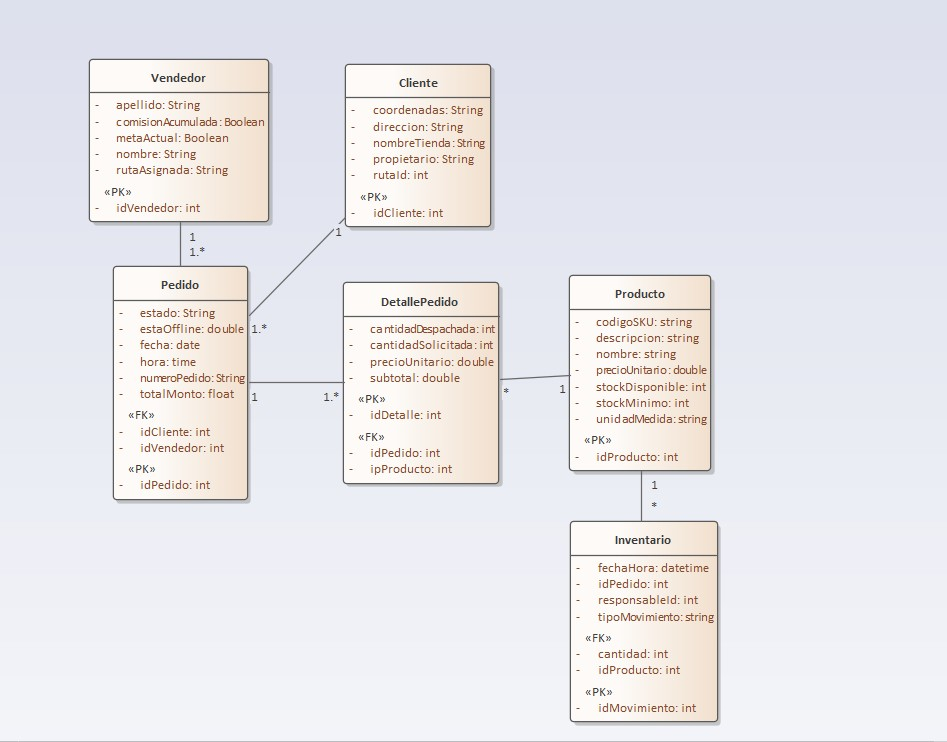
\includegraphics[width=0.9\textwidth]{Diagrama_BD.jpg}
		\caption{Diagrama Lógico de Base de Datos para Django}
		\label{fig:diagrama_bd}
	\end{figure}
	La Figura \ref{fig:diagrama_bd} representa la estructura física adaptada para Django. En este diagrama se visualizan las Llaves Primarias (\texttt{<<PK>>}) y Llaves Foráneas (\texttt{<<FK>>}) que garantizan la integridad referencial entre los perfiles de usuario, catálogos de proveedores y las transacciones de pedidos.
	
	\section{Diagrama de componentes}
	El sistema distribuye sus funcionalidades en tres capas principales que agrupan los componentes de software, garantizando el aislamiento de responsabilidades y la escalabilidad del proyecto.
	
	\begin{figure}[H]
		\centering
		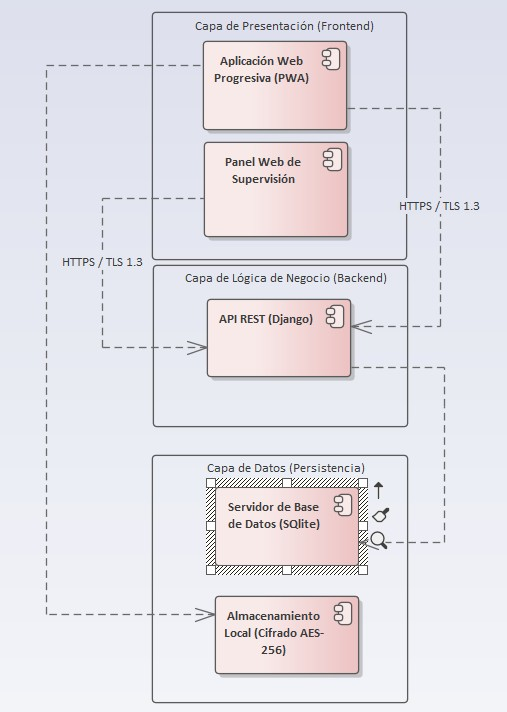
\includegraphics[width=0.9\textwidth]{Dgm_Componentes.jpg}
		\caption{Diagrama de Componentes (Arquitectura en 3 Capas)}
		\label{fig:diagrama_componentes}
	\end{figure}
	En la Figura \ref{fig:diagrama_componentes} se ilustra la arquitectura orientada a servicios del sistema GIRO. La \textbf{Capa de Presentación} contiene la interfaz web responsiva para los vendedores en ruta y los paneles de control web para los proveedores mayoristas. Estos componentes se comunican de forma segura (mediante HTTPS / TLS 1.3) con la \textbf{Capa de Lógica de Negocio}, donde la API desarrollada en Django procesa las peticiones, validaciones de perfiles y reglas de negocio. Finalmente, la \textbf{Capa de Datos} garantiza la persistencia centralizada mediante el servidor MariaDB.
	
	\section{Arquitectura lógica y física (propuesta)}
	El sistema GIRO adopta una arquitectura orientada a servicios, diseñada para alta disponibilidad y el manejo de contextos con baja conectividad:
	\begin{itemize}
		\item \textbf{Arquitectura Lógica:} El frontend opera como una aplicación web con capacidades \textit{offline-first}, sincronizando datos asíncronamente con el backend. Este último expone servicios que centralizan la lógica de validación de stock y el control de solicitudes comerciales.
		\item \textbf{Arquitectura Física:} Los usuarios acceden mediante navegadores web desde smartphones o computadoras de escritorio. El servidor web y la base de datos se alojan en una infraestructura en la nube que permite el escalamiento horizontal, garantizando un \textit{uptime} del 99.5\%.
	\end{itemize}
	
	\section{Prototipo de pantallas no funcional}
	Las interfaces web están diseñadas con un enfoque responsivo para adaptarse a pantallas móviles, cumpliendo con la restricción de diseño de botones táctiles amplios para el uso ágil en campo. A continuación, se presenta el flujo principal para la toma de pedidos.
	
	\begin{figure}[H]
		\centering
		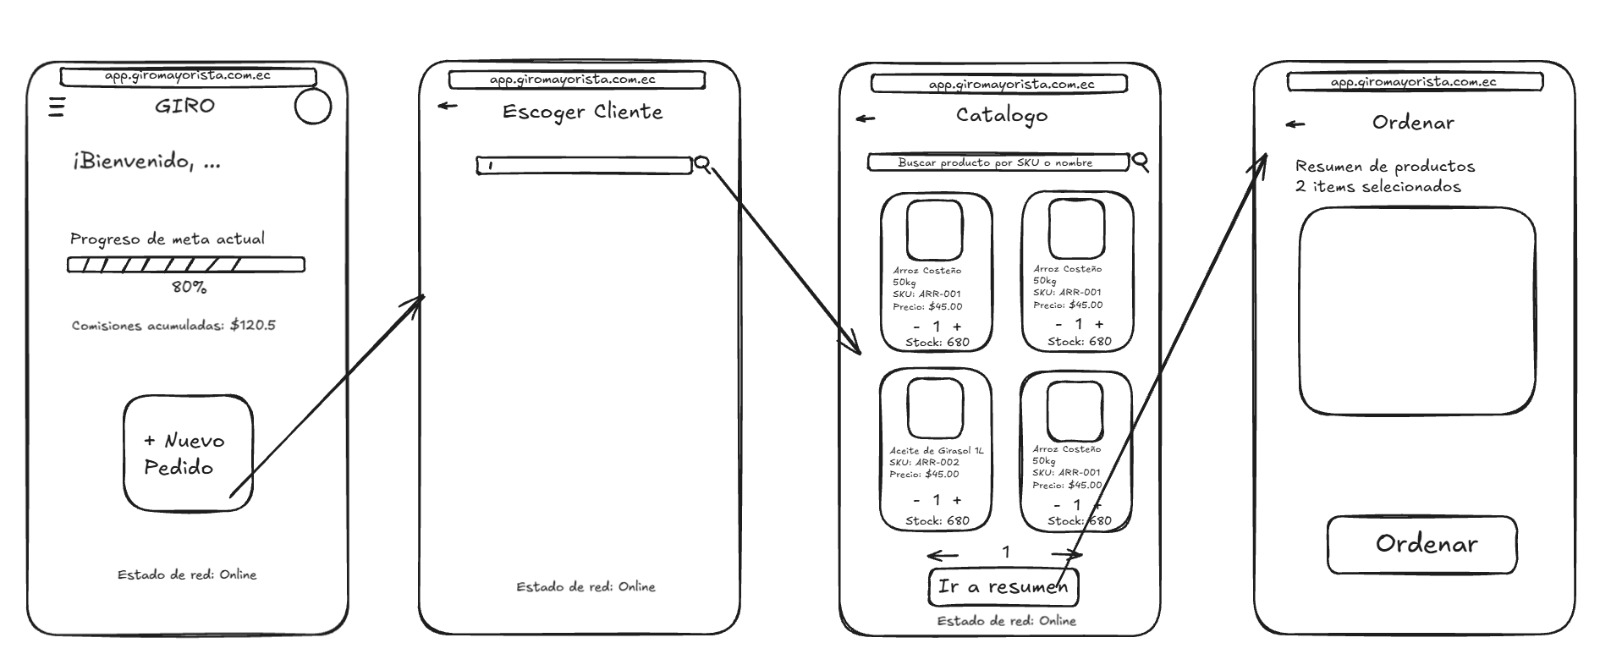
\includegraphics[width=\textwidth]{Wireframe_venta_Ruta.jpeg}
		\caption{Wireframe del Flujo de Venta en Ruta (PWA)}
		\label{fig:wireframe_venta}
	\end{figure}
	
	La Figura \ref{fig:wireframe_venta} detalla el prototipo de la secuencia de pantallas que utiliza el vendedor durante su ruta:
	\begin{itemize}
		\item \textbf{Dashboard (Inicio):} Presenta un resumen del rendimiento del vendedor (progreso de meta actual y comisiones acumuladas) junto con accesos directos para la gestión de pedidos.
		\item \textbf{Escoger Cliente:} Una interfaz limpia equipada con una barra de búsqueda que permite filtrar y seleccionar rápidamente el micromercado a gestionar.
		\item \textbf{Catálogo:} Despliega los productos disponibles del proveedor asociado en formato de tarjetas, indicando su SKU, precio y \textit{stock} actualizado. Incluye selectores numéricos de cantidades y un botón para avanzar al resumen.
		\item \textbf{Ordenar (Resumen):} Pantalla final que muestra la consolidación de los ítems seleccionados y el método de pago antes de confirmar el envío hacia el sistema del proveedor mayorista.
	\end{itemize}
	
\end{document}